\documentclass[a4paper]{article}

\usepackage{polyglossia}
\setdefaultlanguage{russian}
\usepackage{fontspec}
\setmainfont{Times New Roman}
\newfontfamily\cyrillicfont{Times New Roman}
\newfontfamily\cyrillicfonttt{FreeMono}

\usepackage{graphicx}
\usepackage{float}
\usepackage{wrapfig}
\usepackage{tikz}
\usepackage{svg}

\usepackage{amsmath, amssymb}

\usepackage{hyperref}
\definecolor{urlcolor}{rgb}{0,0,1}
\definecolor{linkcolor}{rgb}{0,0,0.8}
\hypersetup{
  pdfborder=0 0 0,
  pdfstartview=FitH,
  linkcolor=linkcolor,
  urlcolor=urlcolor,
  colorlinks=true
}

\usepackage{caption}
\usepackage{geometry}
\geometry{left=2cm, right=2cm, top=2cm, bottom=2cm}

\usepackage{fancyhdr}
\usepackage{nicefrac}

\usepackage{xcolor}
\definecolor{strings}{rgb}{0,0.6,0}
\definecolor{comments}{rgb}{0,0.3,0}
\definecolor{numbers}{rgb}{0.5,0.5,0.5}
\definecolor{keywords}{rgb}{0.09,0.61,0.95}
\definecolor{background}{rgb}{0.97,0.97,0.97}

\usepackage{listings}

\lstdefinestyle{codestyle}{
    backgroundcolor=\color{background},
    commentstyle=\color{comments},
    keywordstyle=\color{keywords},
    stringstyle=\color{strings},
    numberstyle=\tiny\color{numbers},
    basicstyle=\ttfamily\footnotesize,
    breakatwhitespace=false,
    breaklines=true,
    captionpos=b,
    inputencoding=utf8,
    keepspaces=true,
    numbers=left,
    numbersep=5pt,
    showspaces=false,
    showstringspaces=false,
    showtabs=false,
    tabsize=2,
    extendedchars=true,
    literate=
      {а}{{\cyra}}1 {б}{{\cyrb}}1 {в}{{\cyrv}}1 {г}{{\cyrg}}1
      {д}{{\cyrd}}1 {е}{{\cyre}}1 {ж}{{\cyrzh}}1 {з}{{\cyrz}}1
      {и}{{\cyri}}1 {й}{{\cyrishrt}}1 {к}{{\cyrk}}1 {л}{{\cyrl}}1
      {м}{{\cyrm}}1 {н}{{\cyrn}}1 {о}{{\cyro}}1 {п}{{\cyrp}}1
      {р}{{\cyrr}}1 {с}{{\cyrs}}1 {т}{{\cyrt}}1 {у}{{\cyru}}1
      {ф}{{\cyrf}}1 {х}{{\cyrh}}1 {ц}{{\cyrc}}1 {ч}{{\cyrch}}1
      {ш}{{\cyrsh}}1 {щ}{{\cyrshch}}1 {ъ}{{\cyrhrdsn}}1 {ы}{{\cyrery}}1
      {ь}{{\cyrsftsn}}1 {э}{{\cyrerev}}1 {ю}{{\cyryu}}1 {я}{{\cyrya}}1
      {А}{{\CYRA}}1 {Б}{{\CYRB}}1 {В}{{\CYRV}}1 {Г}{{\CYRG}}1
      {Д}{{\CYR96}}1 {Е}{{\CYRE}}1 {Ж}{{\CYRZH}}1 {З}{{\CYRZ}}1
      {И}{{\CYRI}}1 {Й}{{\CYRISHRT}}1 {К}{{\CYRK}}1 {Л}{{\CYRL}}1
      {М}{{\CYRM}}1 {Н}{{\CYRN}}1 {О}{{\CYRO}}1 {П}{{\CYRP}}1
      {Р}{{\CYRR}}1 {С}{{\CYRS}}1 {Т}{{\CYRT}}1 {У}{{\CYRU}}1
      {Ф}{{\CYRF}}1 {Х}{{\CYRH}}1 {Ц}{{\CYRC}}1 {Ч}{{\CYRCH}}1
      {Ш}{{\CYRSH}}1 {Щ}{{\CYRSHCH}}1 {Ъ}{{\CYRHRDSN}}1 {Ы}{{\CYRERY}}1
      {Ь}{{\CYRSFTSN}}1 {Э}{{\CYREREV}}1 {Ю}{{\CYRYU}}1 {Я}{{\CYRYA}}1
}

\lstset{style=codestyle}

\newcommand{\addsection}[1]{
    \phantomsection
    \addcontentsline{toc}{section}{#1}
    \section*{#1}
}
\newcommand{\addsubsection}[1]{
    \phantomsection
    \addcontentsline{toc}{subsection}{#1}
    \subsection*{#1}
}
\newcommand{\addsubsubsection}[1]{
    \phantomsection
    \addcontentsline{toc}{subsubsection}{#1}
    \subsubsection*{#1}
}

\begin{document}

\begin{titlepage}
    \centering
    {\large Федеральное государственное автономное образовательное учреждение\par}
    {\large высшего образования\par}
    {\bfseries САНКТ-ПЕТЕРБУРГСКИЙ НАЦИОНАЛЬНЫЙ ИССЛЕДОВАТЕЛЬСКИЙ УНИВЕРСИТЕТ ИТМО\par}
    {\bfseries Факультет систем управления и робототехники\par}
    \vfill
    {\Large \bfseries Лабораторная работа №6\par}
    {\Large \bfseries Обработка изображений\par}
    \vfill
    
    \begin{flushright}
        Студент: Сайфуллин Д.Р. \\
        Поток: ЧАСТ.МЕТ. R23 1.5 \\ 
        Преподаватели: Перегудин А.А.\\
        Догадин  Е.В.
    \end{flushright}
    \vfill
    Санкт-Петербург \\
    2025 г.
\end{titlepage}

\tableofcontents
\newpage

\addsection{Задание 1. Фильтрация изображений с периодичностью}
В этом задание мы попробуем удалить нежелательные периодические артефакты на изображении путём анализа его Фурье-спектра и удаления ярких гармоник.

Для выполнения задания возьмем одно из предложенных изображений. Я взял изображение \texttt{13.png} и посмотрим на нее:

\begin{figure}[H]
      \centering
      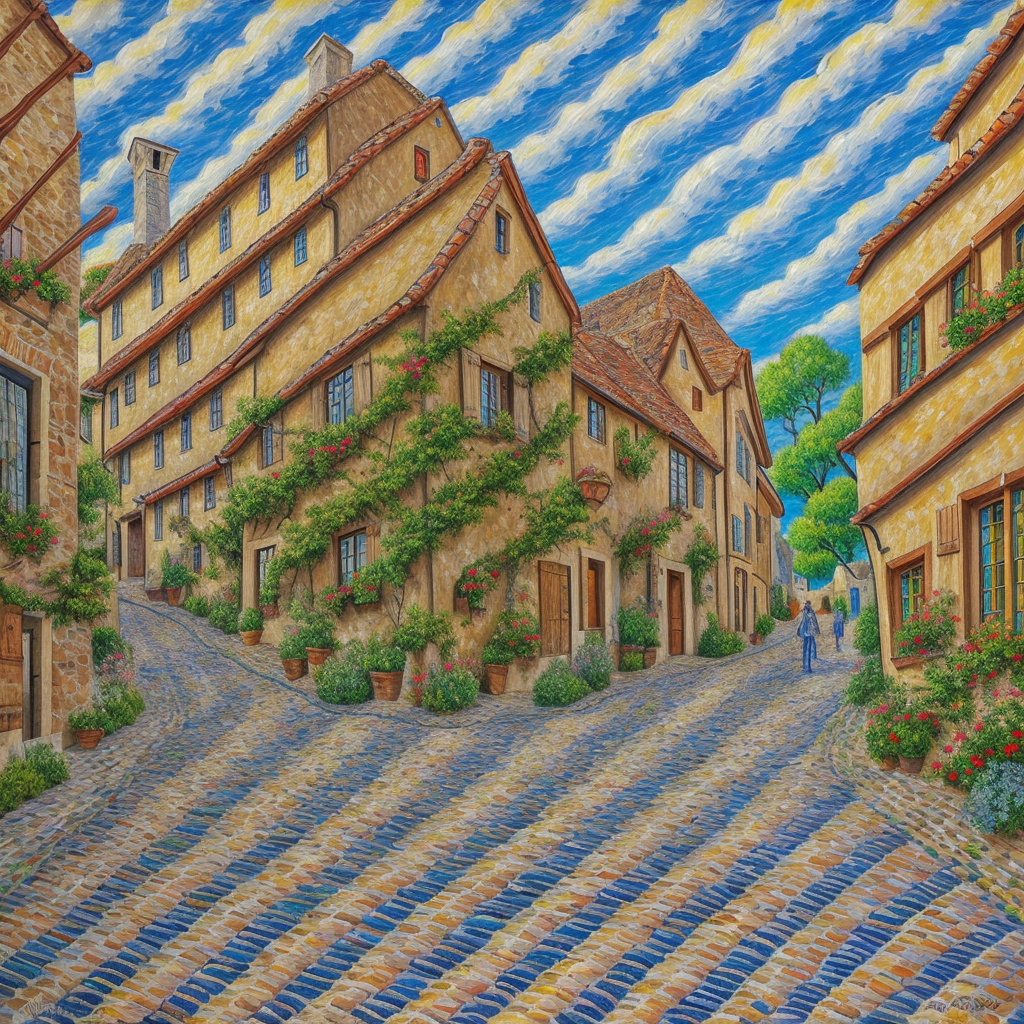
\includegraphics[width=0.6\textwidth]{src/13.png}
      \caption{Исходное изображение.}
\end{figure}

\noindent Мы видим на изображении волны, которые проявляются в виде вертикальных полос. Для их удаления мы воспользуемся Фурье-преобразованием. Поделим все значения в массиве на 255, применим логарифмирование, сдвинем график и найдем его Фурье-преобразование. После этого мы получим Фурье-спектр изображения. Посмотрим на него:
\begin{figure}[H]
      \centering
      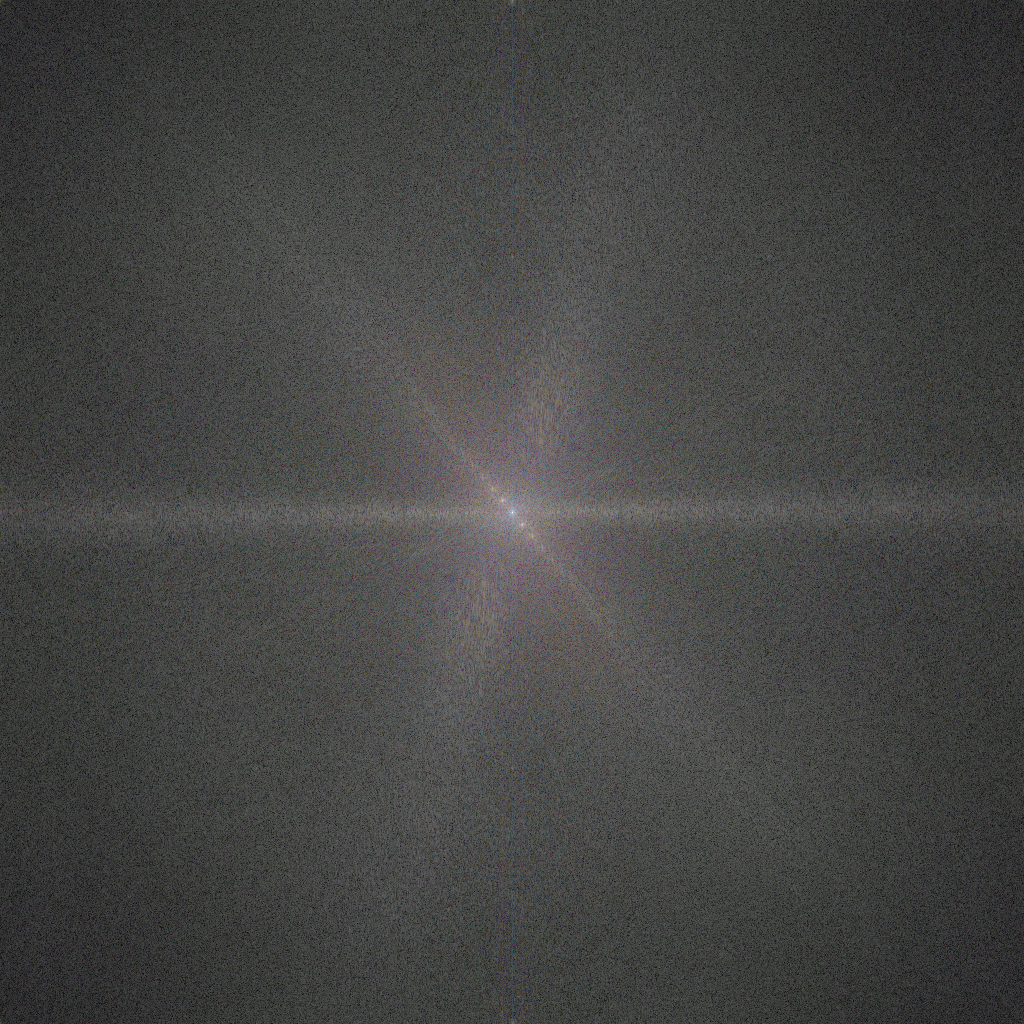
\includegraphics[width=0.6\textwidth]{src/spec_orig.png}
      \caption{Фурье-спектр изображения.}
\end{figure}

\noindent На графике мы видим, что в районе центра изображения есть яркие точки, которые указывают на наличие нежелательных гармоник. Попробуем сгладить цветовые пики, отвечающие за гармоники, с помощью редактора изображений. 

\begin{figure}[H]
  \centering
  \includegraphics[width=0.6\textwidth]{src/spec_filtered.png}
  \caption{Отредактированный Фурье-спектр изображения.}
\end{figure}

\noindent На графике мы видим, что мы удалили нежелательные гармоники. Теперь попробуем восстановить изображение. Для этого применим обратное Фурье-преобразование к отредактированному Фурье-спектру. Используем сохраненную фазу и максимальное значение амплитуды, чтобы восстановить изображение. После этого мы получим отфильтрованное изображение. Посмотрим на результат: 

\begin{figure}[H]
  \centering
  \begin{minipage}{0.49\textwidth}
    \centering
    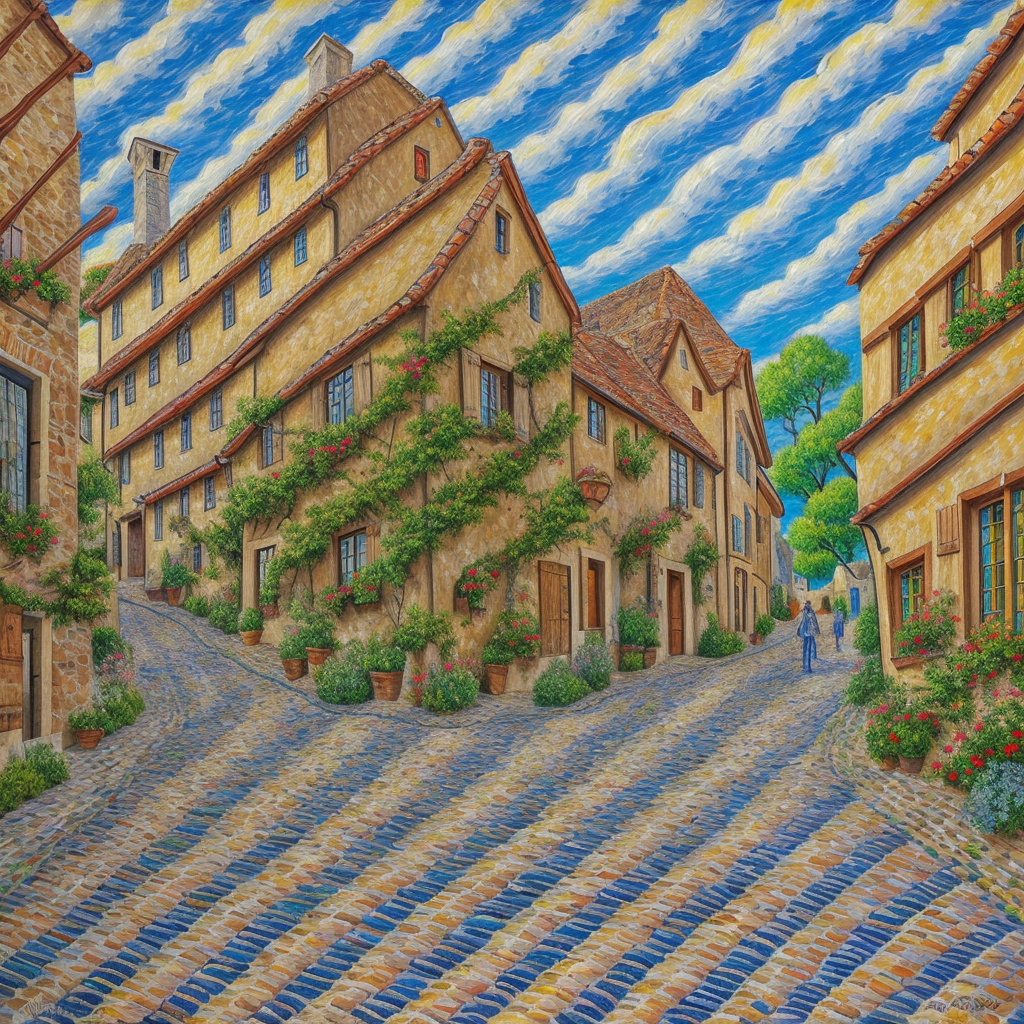
\includegraphics[width=\textwidth]{src/13.png}
    \caption{Исходное изображение.}  
  \end{minipage}
  \begin{minipage}{0.49\textwidth}
    \centering
    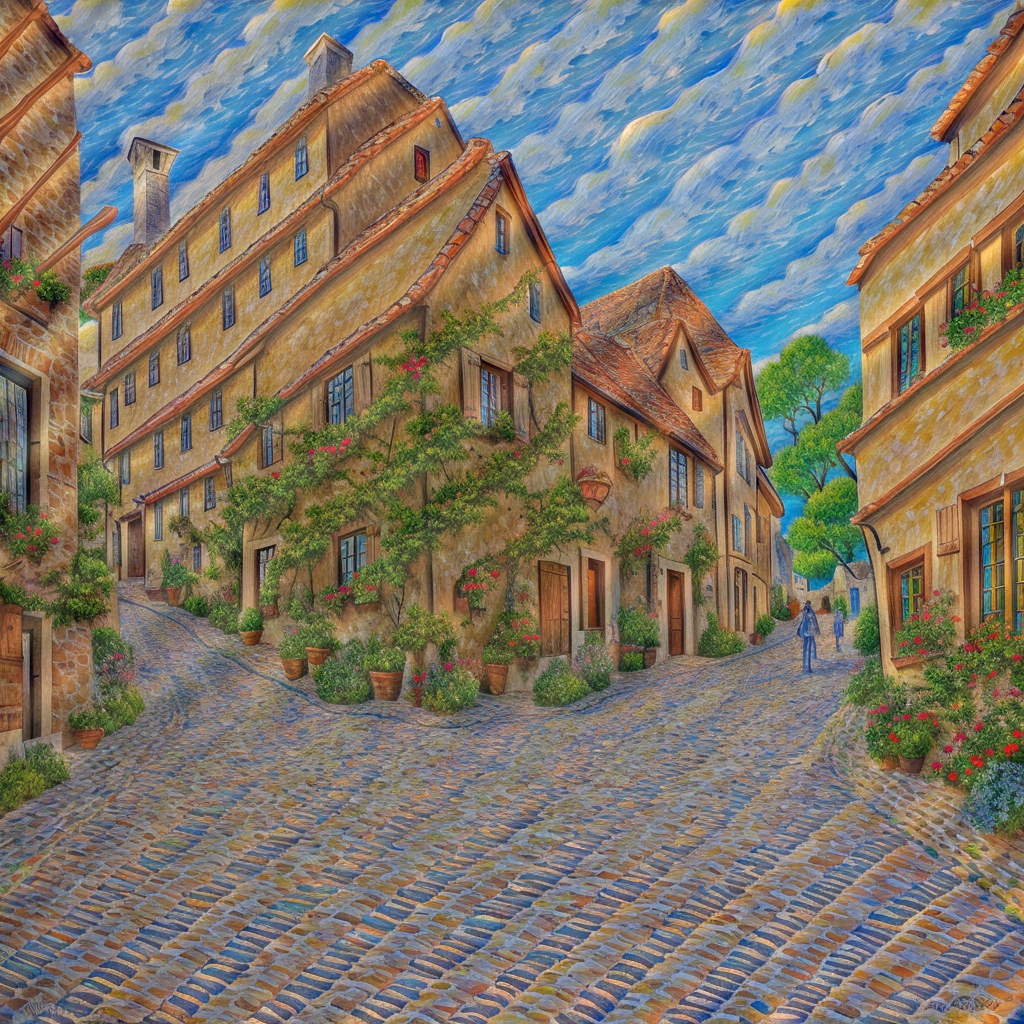
\includegraphics[width=\textwidth]{src/filtered.png}
    \caption{Отфильтрованное изображение.}  
  \end{minipage}
\end{figure}

\noindent У нас получилось. Мы смогли удалить нежелательные гармоники на изображении. Теперь изображение выглядит более четким и ясным.

\paragraph{Выводы}
\begin{itemize}
  \item Лог-спектр позволяет наглядно выявить периодические помехи в виде ярких пикселей вне центра.
  \item Ручная чистка гармоник в сочетании с реконструкцией по сохранённой фазе эффективно подавляет артефакты.
  \item Итоговое изображение сохраняет цветовую гамму и детали, лишившись периодических шумов.
\end{itemize}

\addsection{Задание 2. Исследование свёртки}
В этом задании мы попробуем исследовать свёртку и её применение в обработке изображений. Для начала выберем изображение, над которым будем ставить эксперименты. Посмотрим на него:

\begin{figure}[H]
  \centering
  
\includegraphics[width=0.6\textwidth]{src/fox.png}
  \caption{Исходное изображение.}
\end{figure}

\noindent Переведем изображение в ЧБ формат. После этого мы получим изображение в градациях серого. Построим также его Фурье-спектр:

\begin{figure}[H]
  \centering
  
\includegraphics[width=0.6\textwidth]{src/grayscale.png}
  \caption{Исходное изображение в ЧБ.}
\end{figure}

\begin{figure}[H]
  \centering
  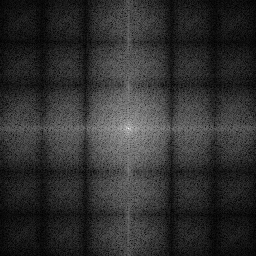
\includegraphics[width=0.6\textwidth]{src/spec_pixel.png}
  \caption{Спектр изображения.}
\end{figure}

Мы будем использовать свёртку с разными фильтрами, чтобы изменять исходное изображение. Будем применять фильтры 2 способами: \texttt{cv2.filter2D()} из OpenCV и поэлементное произведение образа изображения и образа ядра, дополненное нулями.

Рассмотрим несколько ядер свёртки, с которыми будем работать:
\begin{itemize}
  \item Размытие по Гауссу:
    \[
      \sigma=\frac{N-1}{6},\quad
      A_{ij}=\exp\Bigl(-\frac{(i-(N+1)/2)^2+(j-(N+1)/2)^2}{2\sigma^2}\Bigr), \quad i, j \in \{1,\, \dots,\, N\} 
    \]
    \[
      K_\sigma = \frac{A}{\sum_{i,j} A_{ij}}.
    \]
  \item Блочное размытие: 
    \[A_{ij}=1, \quad i, j \in \{1,\, \dots,\, N\} \quad K_\Box=\frac{A}{\sum_{i,j}A_{ij}}\].
  \item Увеличение резкости:
    \[ K_*=\begin{bmatrix}0&-1&0\\-1&5&-1\\0&-1&0\end{bmatrix}.\]
  \item Выделение краёв:
    \[ K_\nabla=\begin{bmatrix}-1&-1&-1\\-1&8&-1\\-1&-1&-1\end{bmatrix}.\]
  \item Кастомное (Собель-X):
    \[ K_{\mathrm{custom}}=\begin{bmatrix}-1&0&1\\-2&0&2\\-1&0&1\end{bmatrix}.\]
\end{itemize}

Начнем с фильтров размития. Возьмем значение $N=\{9, 15, 49\}$. Теперь попробуем применить свёртку к изображению с помощью фильтров. Посмотрим на результат:

\begin{figure}[H]
  \centering
  \begin{minipage}{0.49\textwidth}
    \centering
    
\includegraphics[width=\textwidth]{src/grayscale.png}
    \caption{Исходное изображение.}  
  \end{minipage}
  \begin{minipage}{0.49\textwidth}
    \centering
    
\includegraphics[width=\textwidth]{src/gauss_9.png}
    \caption{Фильтр Гаусса с \texttt{filter2D()} при $N=9$.}
  \end{minipage}
\end{figure}

\begin{figure}[H]
  \centering
  \begin{minipage}{0.49\textwidth}
    \centering
    
\includegraphics[width=\textwidth]{src/grayscale.png}
    \caption{Исходное изображение.}  
  \end{minipage}
  \begin{minipage}{0.49\textwidth}
    \centering
    
\includegraphics[width=\textwidth]{src/gauss_15.png}
    \caption{Фильтр Гаусса с \texttt{filter2D()} при $N=15$.}
  \end{minipage}
\end{figure}

\begin{figure}[H]
  \centering
  \begin{minipage}{0.49\textwidth}
    \centering
    
\includegraphics[width=\textwidth]{src/grayscale.png}
    \caption{Исходное изображение.}  
  \end{minipage}
  \begin{minipage}{0.49\textwidth}
    \centering
    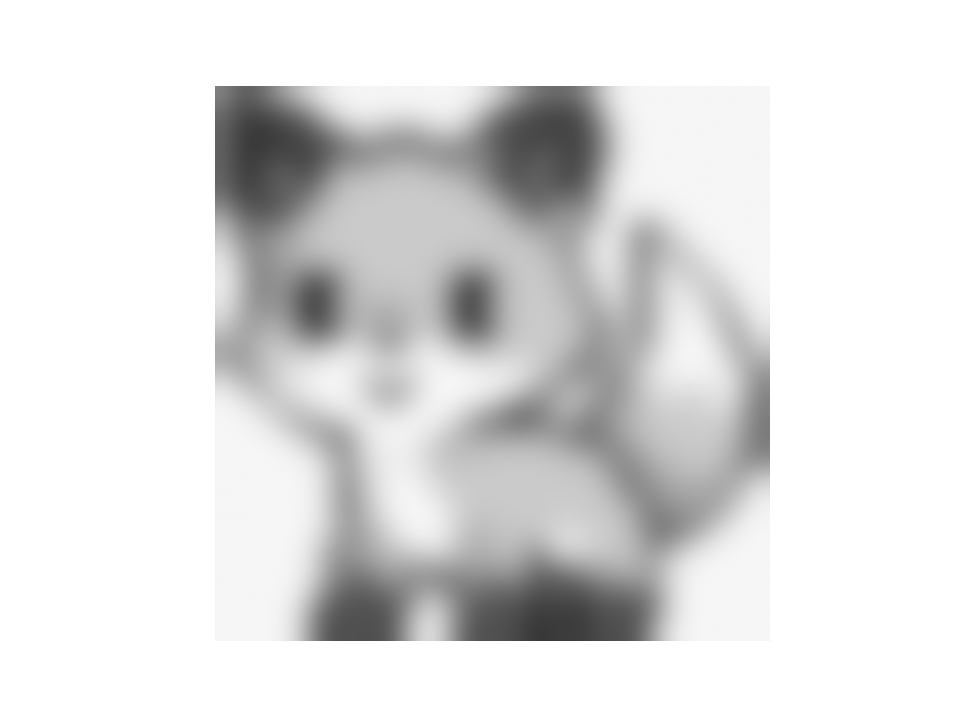
\includegraphics[width=\textwidth]{src/gauss_49.png}
    \caption{Фильтр Гаусса с \texttt{filter2D()} при $N=49$.}
  \end{minipage}
\end{figure}

\noindent Мы видим, что при увеличении значения $N$ изображение становится более размытым. Посмотрим на образы ядер при разных значениях $N$:

\begin{figure}[H]
  \centering
  \includesvg[width=0.4\textwidth]{src/spec_gauss_9.svg}
  \caption{Образ ядра фильтра Гаусса при $N=9$.}
\end{figure}
\begin{figure}[H]
  \centering
  \includesvg[width=0.4\textwidth]{src/spec_gauss_15.svg}
  \caption{Образ ядра фильтра Гаусса при $N=15$.}
\end{figure}
\begin{figure}[H]
  \centering
  \includesvg[width=0.4\textwidth]{src/spec_gauss_49.svg}
  \caption{Образ ядра фильтра Гаусса при $N=49$.}
\end{figure}

\noindent При $N=9$ спектр — яркая центральная точка средних размеров, плавно убывающая. При $N=15$ центральная область сжатее, переход к высоким частотам более резкий.  При $N=49$ наблюдается почти точечный пик в центре.

Теперь попробуем применить тот же фильтр, но вторым способом.

\begin{figure}[H]
  \centering
  \begin{minipage}{0.49\textwidth}
    \centering
    
\includegraphics[width=\textwidth]{src/gauss_9.png}
    \caption{Фильтр Гаусса с \texttt{filter2D()} при $N=9$.}
  \end{minipage}
  \begin{minipage}{0.49\textwidth}
    \centering
    
\includegraphics[width=\textwidth]{src/ifft_gauss_9.png}
    \caption{Фильтр Гаусса через Фурье-образ при $N=9$.}
  \end{minipage}
\end{figure}

\begin{figure}[H]
  \centering
  \begin{minipage}{0.49\textwidth}
    \centering
    
\includegraphics[width=\textwidth]{src/gauss_15.png}
    \caption{Фильтр Гаусса с \texttt{filter2D()} при $N=15$.}
  \end{minipage}
  \begin{minipage}{0.49\textwidth}
    \centering
    
\includegraphics[width=\textwidth]{src/ifft_gauss_15.png}
    \caption{Фильтр Гаусса через Фурье-образ при $N=15$.}
  \end{minipage}
\end{figure}

\begin{figure}[H]
  \centering
  \begin{minipage}{0.49\textwidth}
    \centering
    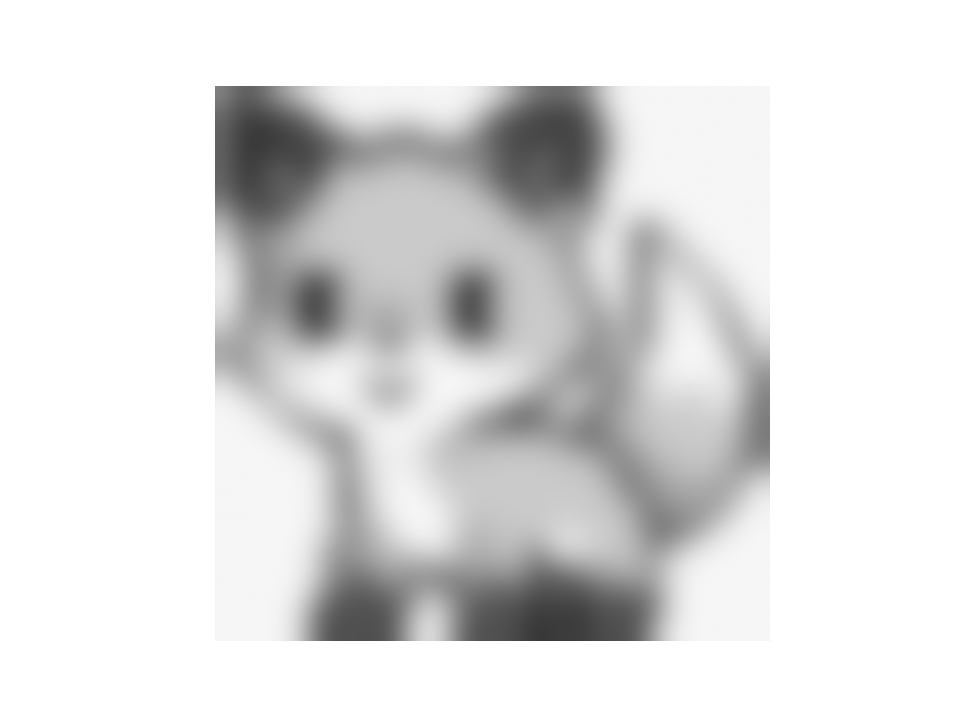
\includegraphics[width=\textwidth]{src/gauss_49.png}
    \caption{Фильтр Гаусса с \texttt{filter2D()} при $N=49$.}
  \end{minipage}
  \begin{minipage}{0.49\textwidth}
    \centering
    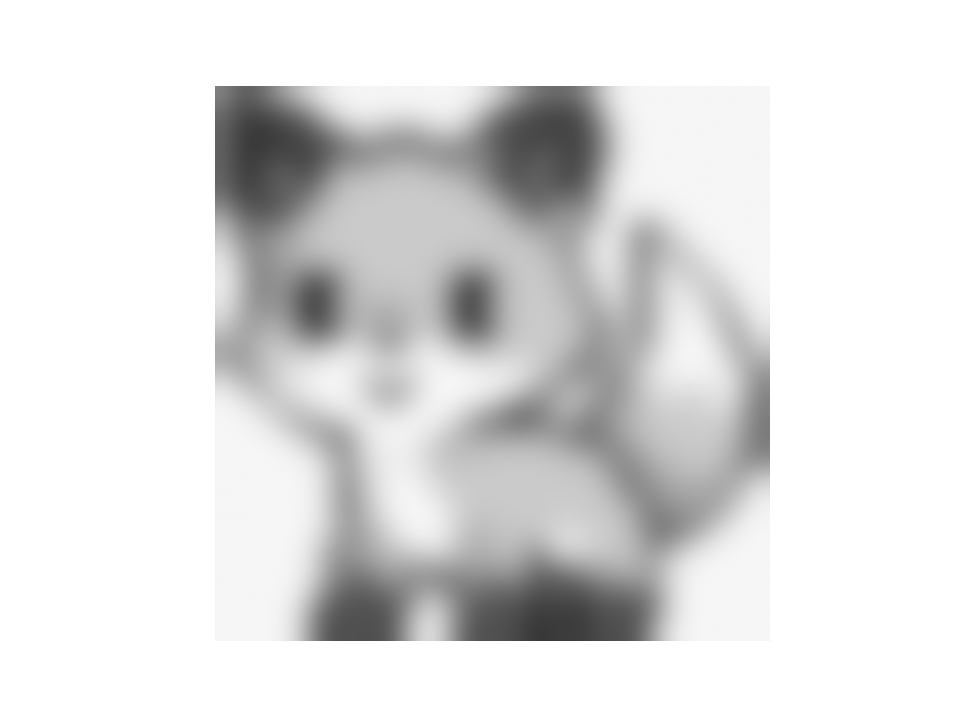
\includegraphics[width=\textwidth]{src/ifft_gauss_49.png}
    \caption{Фильтр Гаусса через Фурье-образ при $N=49$.}
  \end{minipage}
\end{figure}

\noindent В случае с произведением преобразований так же наблюдается размытие изображения при увеличение $N$. Но результат отличался от того, что мы получили с помощью \texttt{cv2.filter2D()} тем, что у изображения появляется черная рамка, которая растет вместе с значениями $N$. Это можно исправить, здесь и в дальнейшем представдены изображения, которые изначально были дополнены с каждой стороны, после этого найдены их Фурье-образы и умножены на образы ядер. По итогу мы получаем полное совпадение в работе двух методов.

Посмотрим на образы отфильтрованных изображений:
\begin{figure}[H]
  \centering
  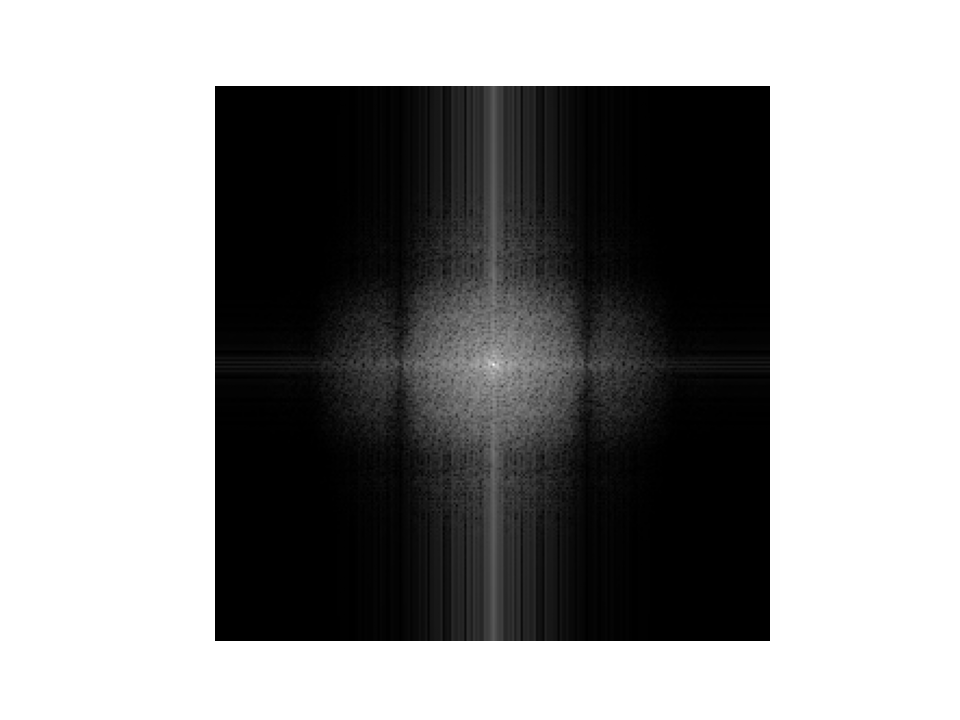
\includegraphics[width=0.4\textwidth]{src/ifft_spec_gauss_9.png}
  \caption{Образ отфильтрованного изображения при $N=9$.}
\end{figure}
\begin{figure}[H]
  \centering
  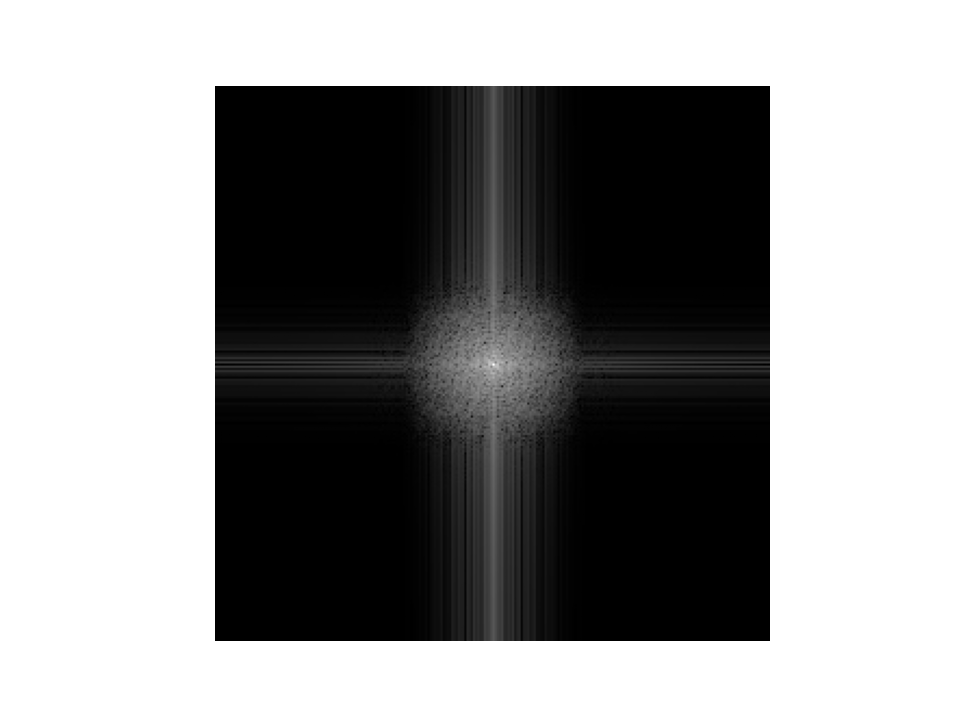
\includegraphics[width=0.4\textwidth]{src/ifft_spec_gauss_15.png}
  \caption{Образ отфильтрованного изображения при $N=15$.}
\end{figure}
\begin{figure}[H]
  \centering
  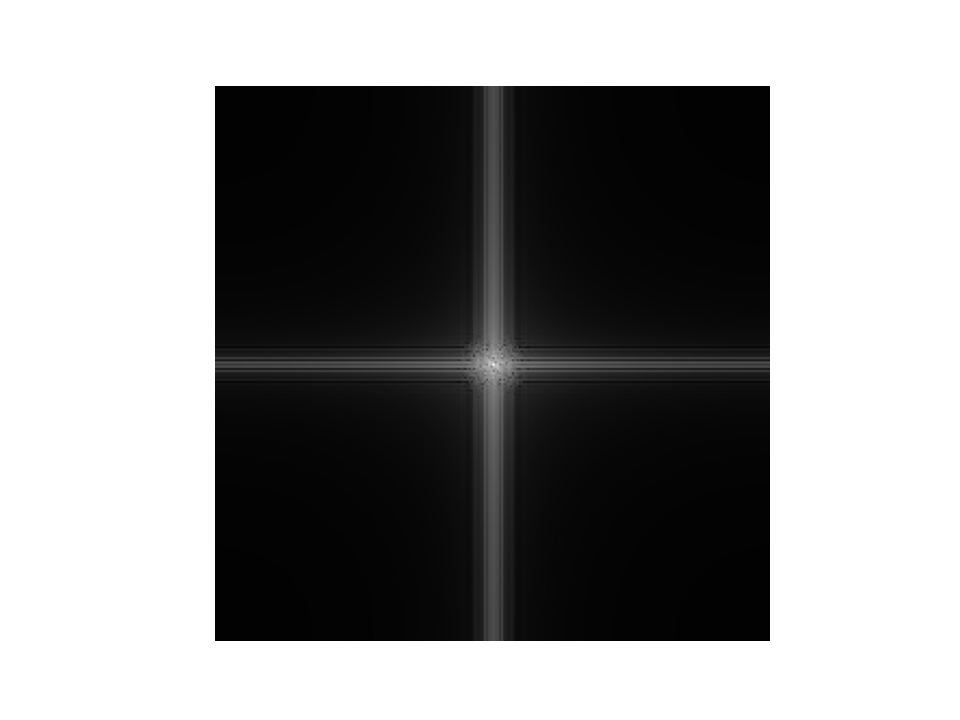
\includegraphics[width=0.4\textwidth]{src/ifft_spec_gauss_49.png}
  \caption{Образ отфильтрованного изображения при $N=49$.}
\end{figure}

\noindent Мы видим как с увеличением $N$ образ фильтрованного изображение стремится к центру. Мы видели такое поведение у образов ядер размытия по Гауссу, следовательно это подтверждает, что фильтр применен правильно.

Далее попробуем посмотреть на блочное размытие: 

\begin{figure}[H]
  \centering
  \begin{minipage}{0.49\textwidth}
    \centering
    
\includegraphics[width=\textwidth]{src/grayscale.png}
    \caption{Исходное изображение.}  
  \end{minipage}
  \begin{minipage}{0.49\textwidth}
    \centering
    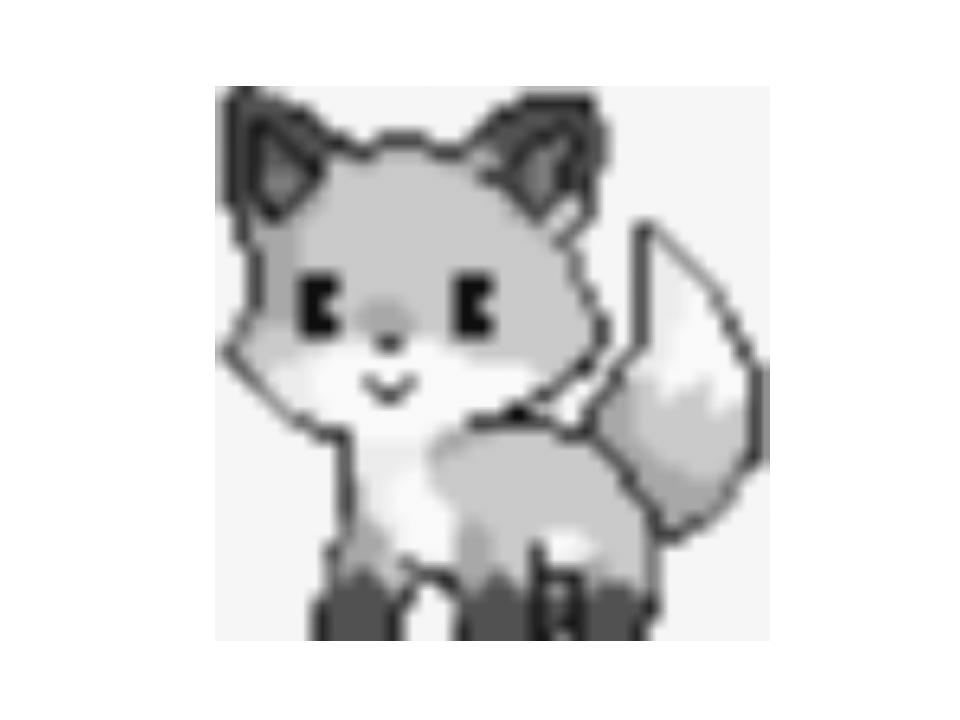
\includegraphics[width=\textwidth]{src/box_9.png}
    \caption{Блочное размытие с \texttt{filter2D()} при $N=9$.}
  \end{minipage}
\end{figure}

\begin{figure}[H]
  \centering
  \begin{minipage}{0.49\textwidth}
    \centering
    
\includegraphics[width=\textwidth]{src/grayscale.png}
    \caption{Исходное изображение.}  
  \end{minipage}
  \begin{minipage}{0.49\textwidth}
    \centering
    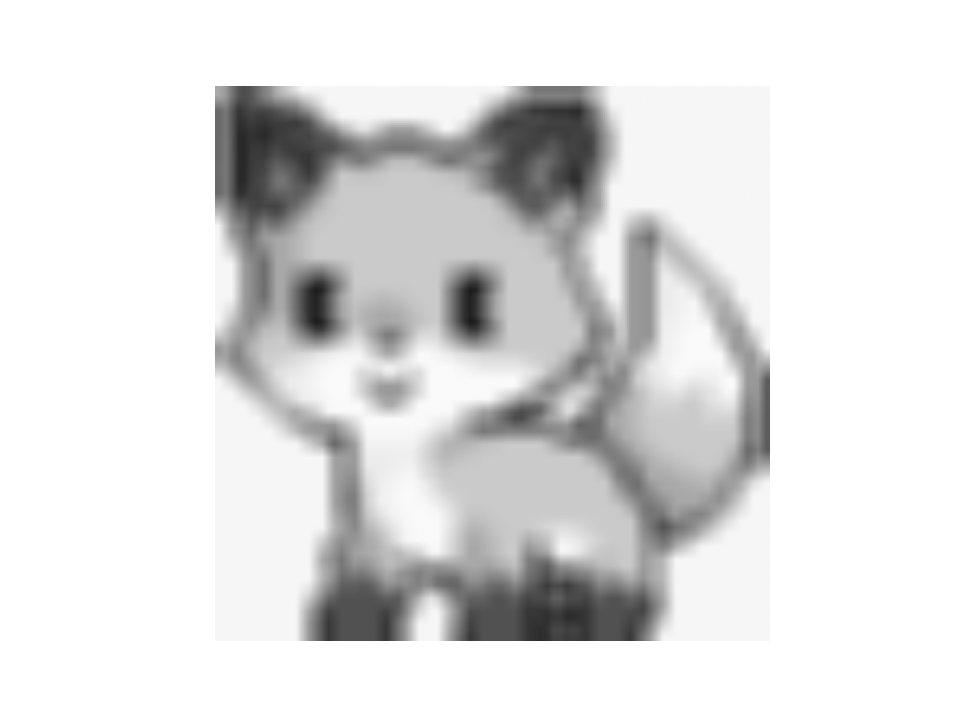
\includegraphics[width=\textwidth]{src/box_15.png}
    \caption{Блочное размытие с \texttt{filter2D()} при $N=15$.}
  \end{minipage}
\end{figure}

\begin{figure}[H]
  \centering
  \begin{minipage}{0.49\textwidth}
    \centering
    
\includegraphics[width=\textwidth]{src/grayscale.png}
    \caption{Исходное изображение.}  
  \end{minipage}
  \begin{minipage}{0.49\textwidth}
    \centering
    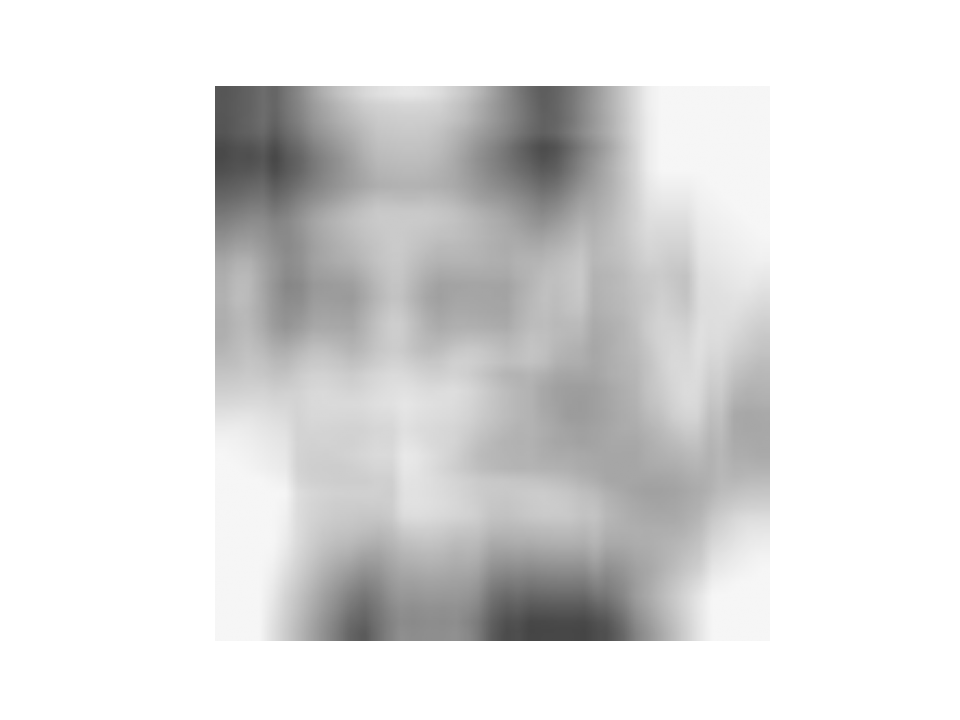
\includegraphics[width=\textwidth]{src/box_49.png}
    \caption{Блочное размытие с \texttt{filter2D()} при $N=49$.}
  \end{minipage}
\end{figure}

\noindent При $N=9$ всё ещё читается форма, но переходы резко ступенчатые, при $N=15$ детали превращаются в прямоугольники, а при $N=49$ изображение наполовину заполнено плоскими областями — края сглажены, но остаются чёткие границы между участками со средней яркостью.

Посмотрим на образы ядер при разных значениях $N$:

\begin{figure}[H]
  \centering
  \includesvg[width=0.4\textwidth]{src/spec_box_9.svg}
  \caption{Образ ядра блочного размытия при $N=9$.}
\end{figure}
\begin{figure}[H]
  \centering
  \includesvg[width=0.4\textwidth]{src/spec_box_15.svg}
  \caption{Образ ядра блочного размытия при $N=15$.}
\end{figure}
\begin{figure}[H]
  \centering
  \includesvg[width=0.4\textwidth]{src/spec_box_49.svg}
  \caption{Образ ядра блочного размытия при $N=49$.}
\end{figure}

\noindent Блочное ядро имеет самое светлое значение в центре. При увелиении размеров эта точка так же уменьшается. Но в отличие от ядра Гаусса, блочное ядро имеет прямоугольные состовляющие на вертикали и горизонтали, а также более резкие границы между участками.

\begin{figure}[H]
  \centering
  \begin{minipage}{0.49\textwidth}
    \centering
    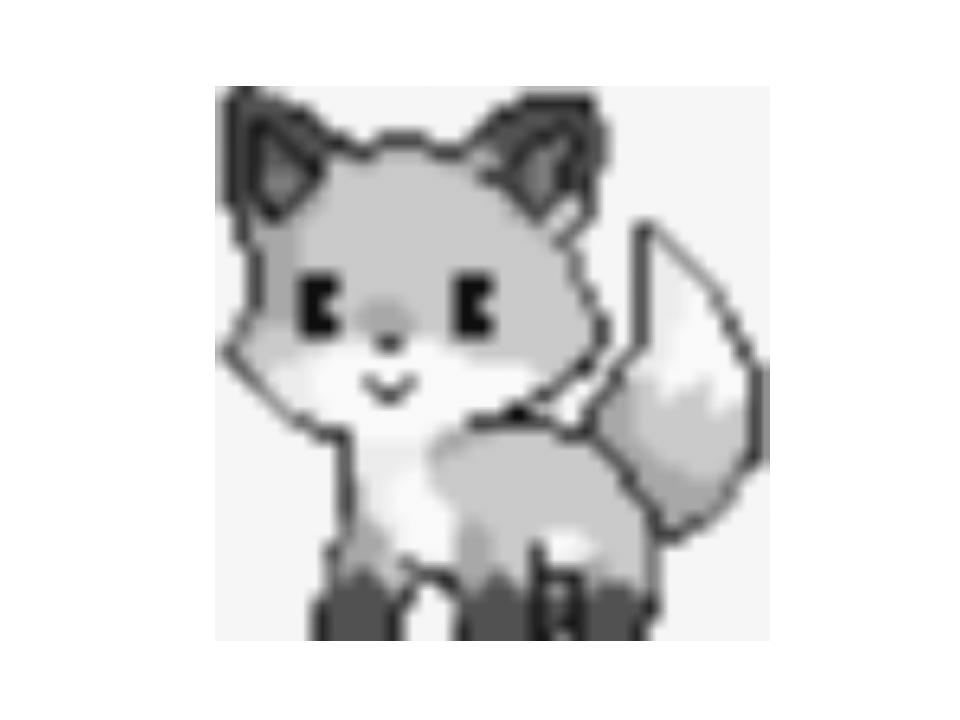
\includegraphics[width=\textwidth]{src/box_9.png}
    \caption{Блочное размытие с \texttt{filter2D()} при $N=9$.}
  \end{minipage}
  \begin{minipage}{0.49\textwidth}
    \centering
    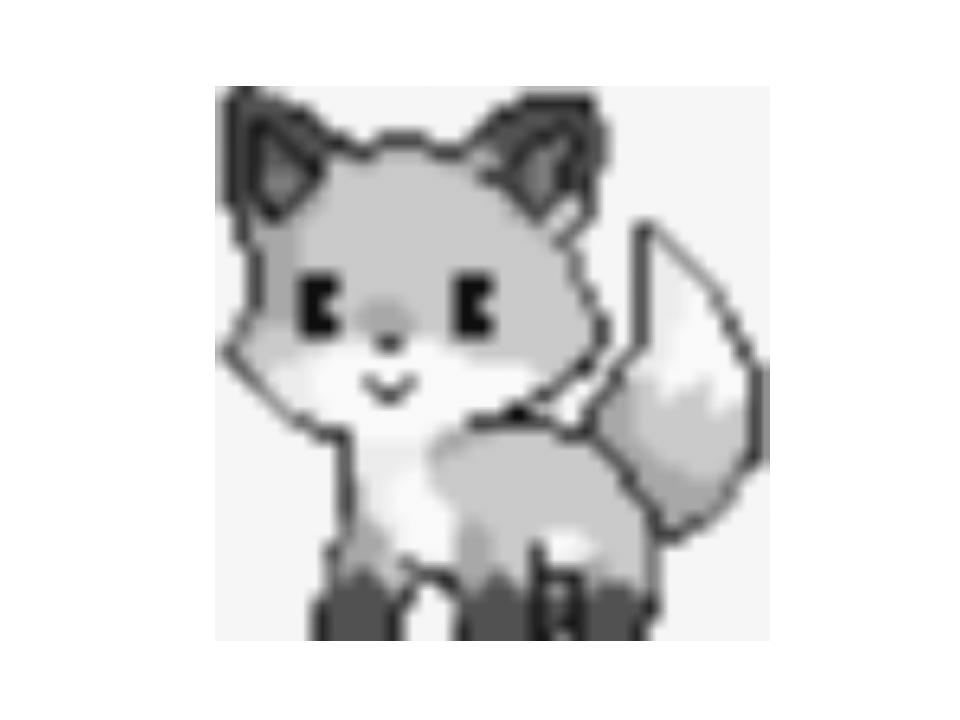
\includegraphics[width=\textwidth]{src/ifft_box_9.png}
    \caption{Блочное размытие через Фурье при $N=9$.}
  \end{minipage}
\end{figure}

\begin{figure}[H]
  \centering
  \begin{minipage}{0.49\textwidth}
    \centering
    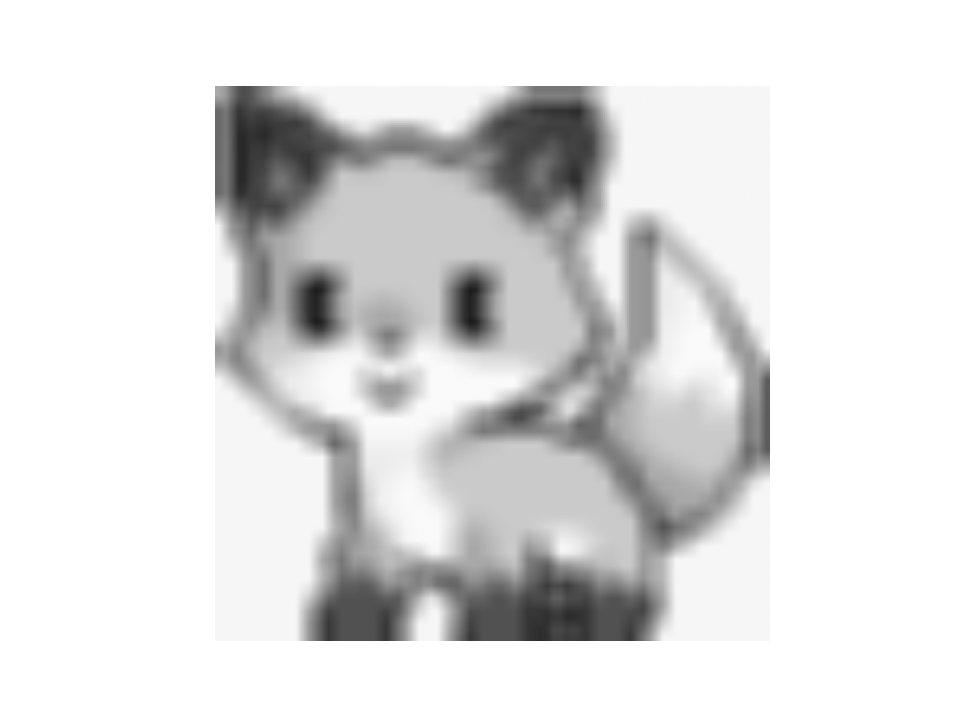
\includegraphics[width=\textwidth]{src/box_15.png}
    \caption{Блочное размытие с \texttt{filter2D()} при $N=15$.}
  \end{minipage}
  \begin{minipage}{0.49\textwidth}
    \centering
    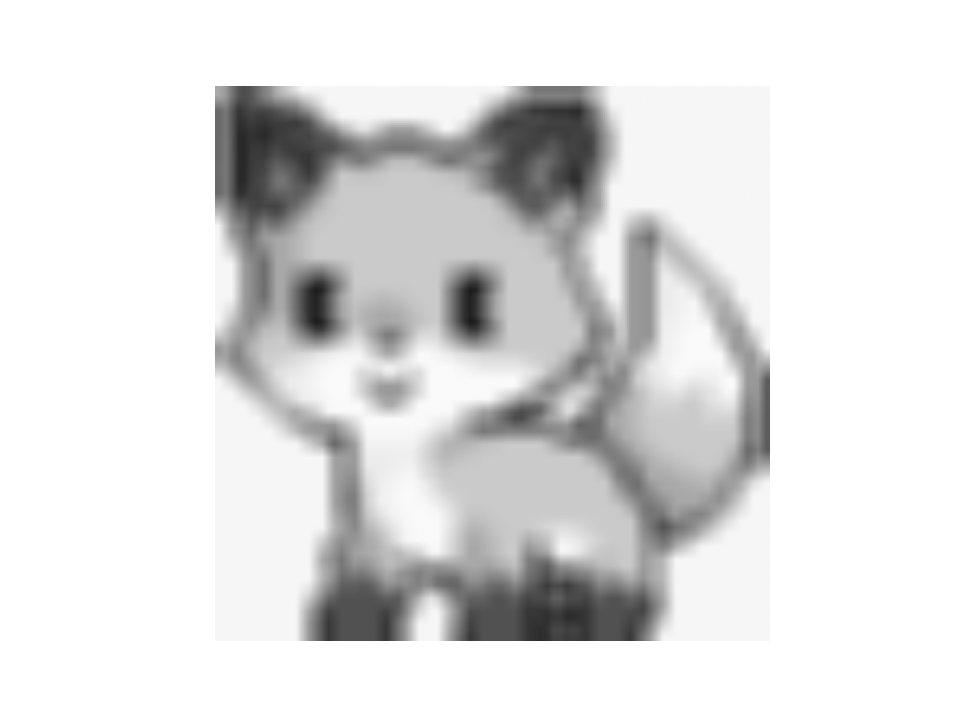
\includegraphics[width=\textwidth]{src/ifft_box_15.png}
    \caption{Блочное размытие через Фурье при $N=15$.}
  \end{minipage}
\end{figure}

\begin{figure}[H]
  \centering
  \begin{minipage}{0.49\textwidth}
    \centering
    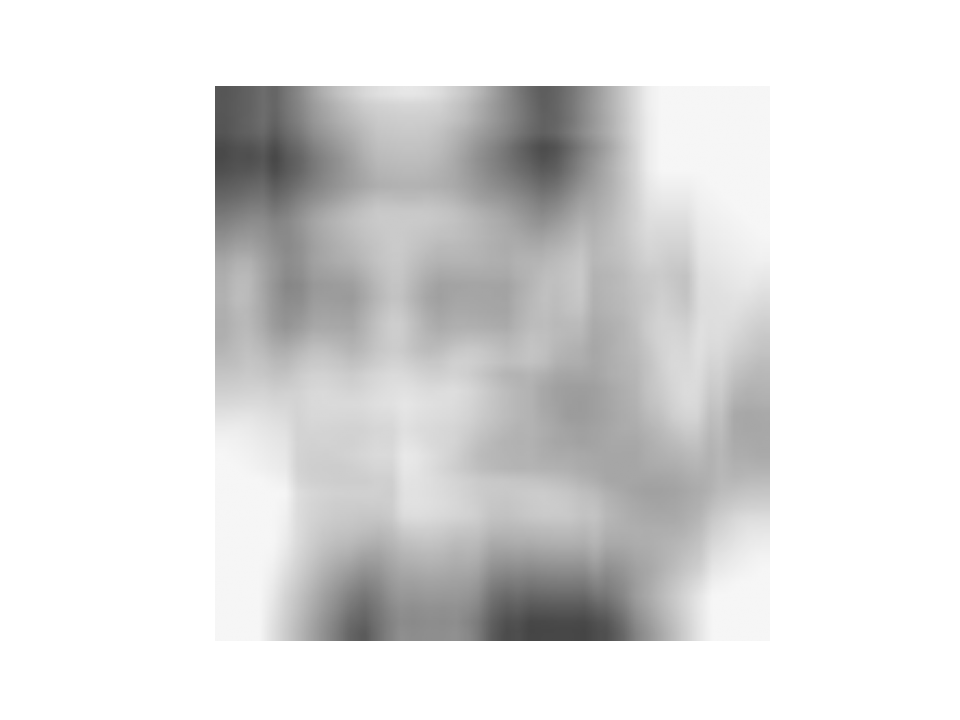
\includegraphics[width=\textwidth]{src/box_49.png}
    \caption{Блочное размытие с \texttt{filter2D()} при $N=49$.}
  \end{minipage}
  \begin{minipage}{0.49\textwidth}
    \centering
    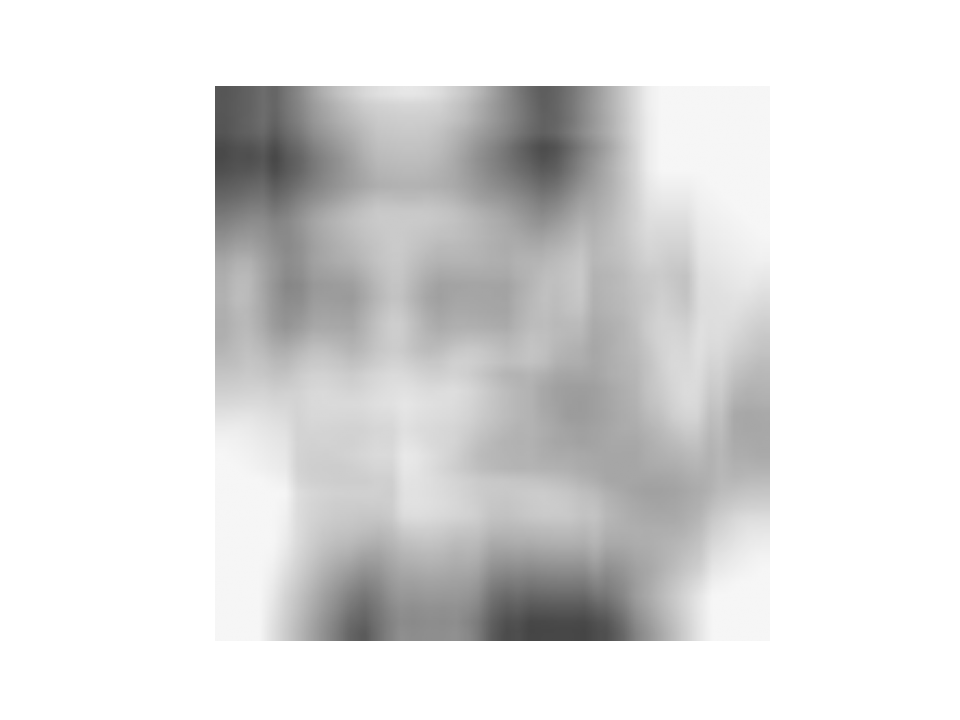
\includegraphics[width=\textwidth]{src/ifft_box_49.png}
    \caption{Блочное размытие через Фурье при $N=49$.}
  \end{minipage}
\end{figure}

\noindent Блочный фильтр усредняет все пиксели в окне $N\times N$ одинаково, создавая «мыльный» эффект с равномерной потерей деталей. В реализации через Фурье-образ мы наблюдаем аналогичное поведение.

Посмотрим на образы отфильтрованных изображений:
\begin{figure}[H]
  \centering
  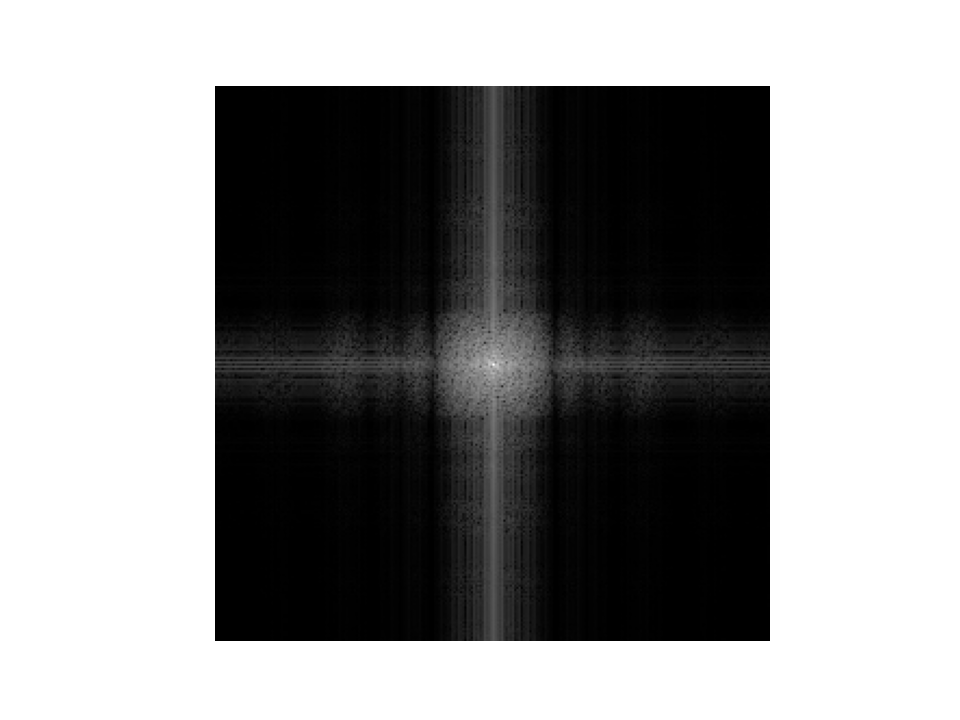
\includegraphics[width=0.4\textwidth]{src/ifft_spec_box_9.png}
  \caption{Образ отфильтрованного изображения при $N=9$.}
\end{figure}
\begin{figure}[H]
  \centering
  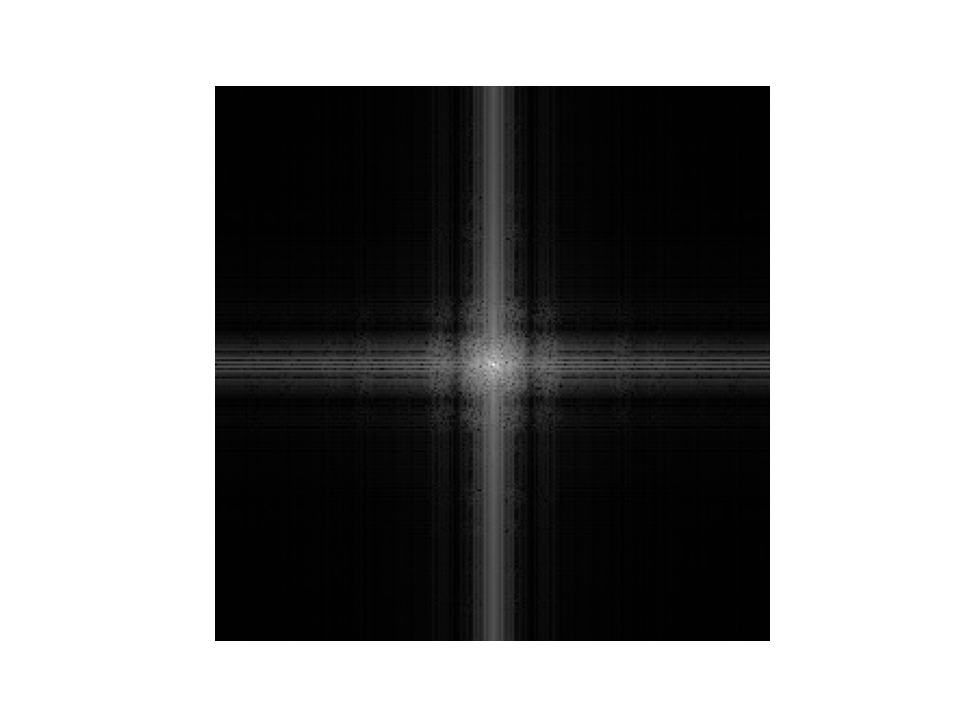
\includegraphics[width=0.4\textwidth]{src/ifft_spec_box_15.png}
  \caption{Образ отфильтрованного изображения при $N=15$.}
\end{figure}
\begin{figure}[H]
  \centering
  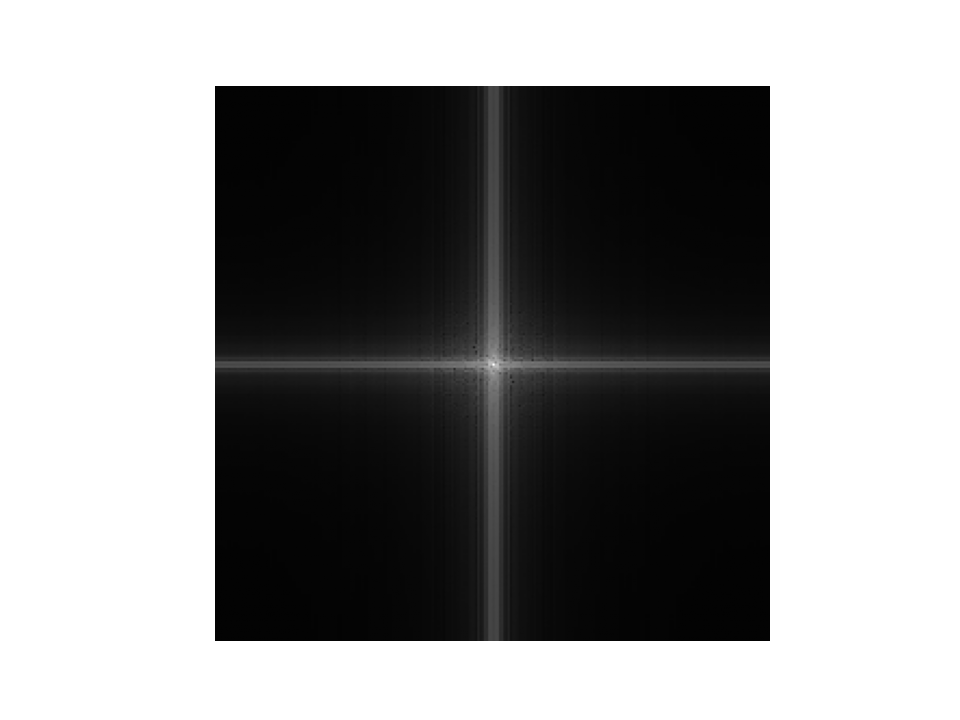
\includegraphics[width=0.4\textwidth]{src/ifft_spec_box_49.png}
  \caption{Образ отфильтрованного изображения при $N=49$.}
\end{figure}

\noindent Мы видим, что при увеличении $N$ самая светлая область образа стремится к центру и уменьшается. При этом вертикальная и горизонтальная полосы деляться на сегменты, которые также уменьшаюся при изменении размеров ядра.

Можем сделать вывод о том, что с увеличением размера ядра гауссово размытие даёт всё более мягкую картинку: переходы между областями интенсивности становятся плавными. Нет никаких характерных следов квадратного окна. Однако при тех же размерах окна блочное размытие сохраняет ступенчатый эффект: картинка разбивается на большие однотонные квадраты, внутри которых все точки усреднены одинаково. В отличие от гаусса, здесь нет радиальной симметрии размытия.

Перейдем к фильтру, который увеличивает резкость изображения. Применим его и посмотрим на результат:

\begin{figure}[H]
  \centering
  \begin{minipage}{0.49\textwidth}
    \centering
    
\includegraphics[width=\textwidth]{src/grayscale.png}
    \caption{Исходное изображение.}  
  \end{minipage}
  \begin{minipage}{0.49\textwidth}
    \centering
    
\includegraphics[width=\textwidth]{src/sharpen.png}
    \caption{Увеличение резкости с \texttt{filter2D()}.}
  \end{minipage}
\end{figure}

\noindent Изображение стало более четким: контуры проявились, а граница квадратов-пикселей стали более явными. Посмотрим на образ ядра фильтра:

\begin{figure}[H]
  \centering
  \includesvg[width=0.4\textwidth]{src/spec_sharpen.svg}
  \caption{Образ ядра резкости.}
\end{figure}

\noindent Мы видим, что ядро резкости имеет темный пик в центре, белые области по углам и плавные границы между ними.

Теперь попробуем применить тот же фильтр, но вторым способом.
\begin{figure}[H]
  \centering
  \begin{minipage}{0.49\textwidth}
    \centering
    
\includegraphics[width=\textwidth]{src/sharpen.png}
    \caption{Увеличение резкости с \texttt{filter2D()}.}
  \end{minipage}
  \begin{minipage}{0.49\textwidth}
    \centering
    
\includegraphics[width=\textwidth]{src/ifft_sharpen.png}
    \caption{Увеличение резкости через Фурье-образ.}
  \end{minipage}
\end{figure}

\noindent Результат аналогичен. Посмотрим на образ отфильтрованного изображения:
\begin{figure}[H]
  \centering
  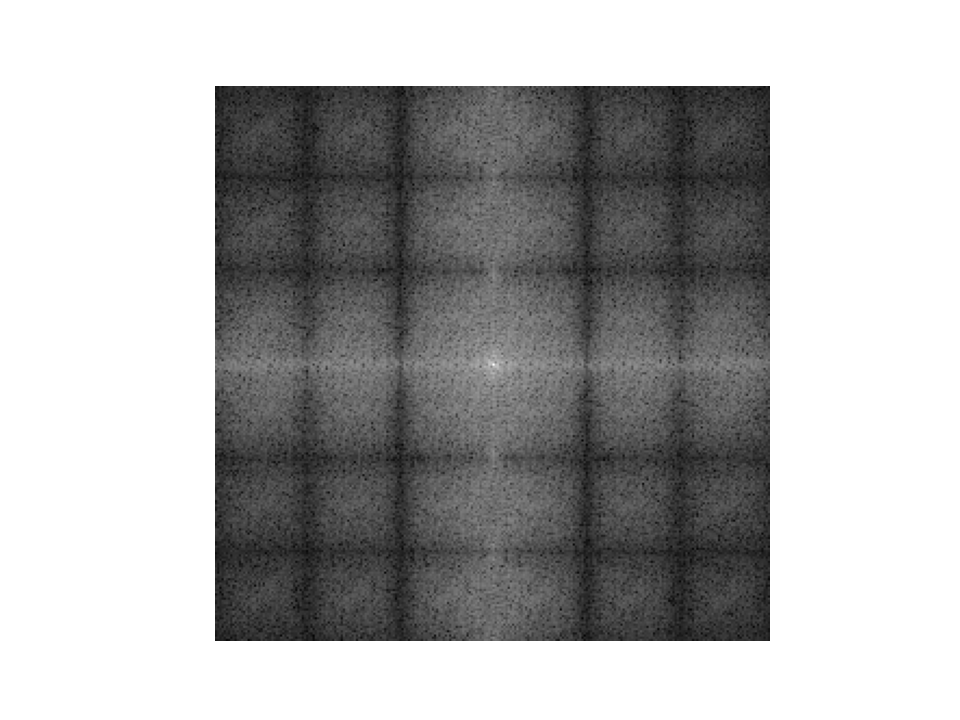
\includegraphics[width=0.4\textwidth]{src/ifft_spec_sharpen.png}
  \caption{Образ отфильтрованного изображения.}
\end{figure}

\noindent Мы видим, что области в углах стали заметно светлее. Это происходит потому что фильтр резкости усиливает высокочастотные компоненты, которые отвечают за резкость изображения.

Теперь попробуем выделить края изображения. Применим фильтр и посмотрим на результат:
\begin{figure}[H]
  \centering
  
\includegraphics[width=0.4\textwidth]{src/grayscale.png}
  \caption{Исходное изображение.}  
  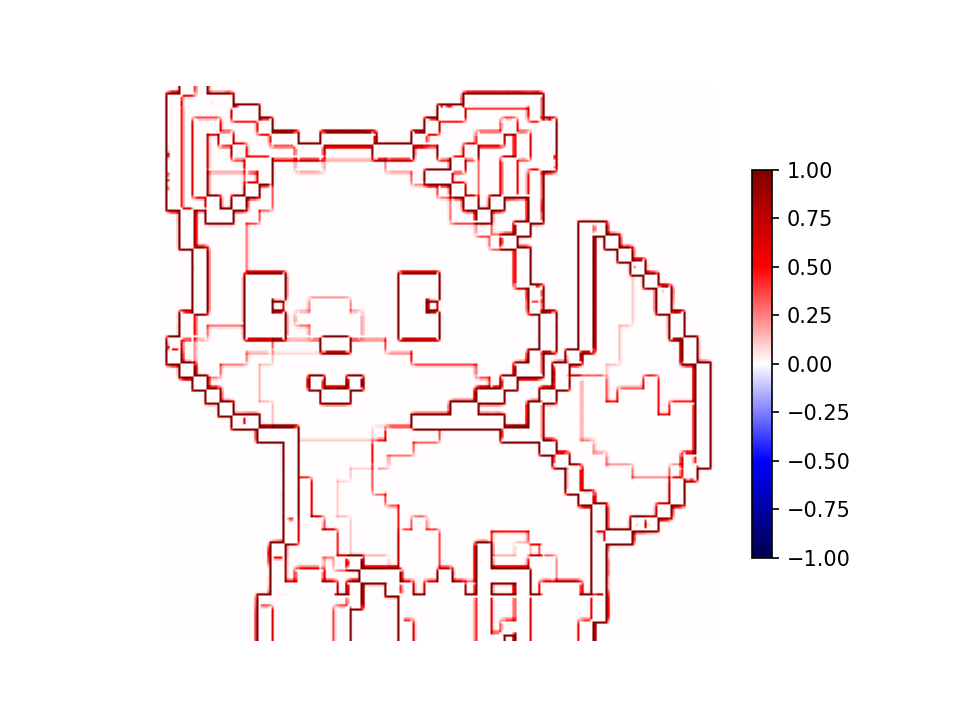
\includegraphics[width=0.7\textwidth]{src/edge.png}
  \caption{Выделение краёв с \texttt{filter2D()}.}
\end{figure}
\noindent Мы видим, что края изображения стали белыми четкими, а все осталальное потеряло свой цвет. Поскольку при применении фильтра выделения краёв значения в выходном изображении могут быть и положительными, и отрицательными, для наглядного их различения мы используем дивергентную (двухцветную) карту:

\begin{itemize}
  \item Красный цвет показывает положительные отклики (границы нарастания яркости);
  \item Синий цвет показывает отрицательные отклики (границы убывания яркости).
\end{itemize}

Посмотрим на образ ядра фильтра:
\begin{figure}[H]
  \centering
  \includesvg[width=0.4\textwidth]{src/spec_edge.svg}
  \caption{Образ ядра выделения краёв.}
\end{figure}
\noindent Мы видим, что ядро выделения краёв имеет темный пик в центре и белые участки в центрах каждой границы.
Теперь попробуем применить тот же фильтр, но вторым способом.
\begin{figure}[H]
  \centering
  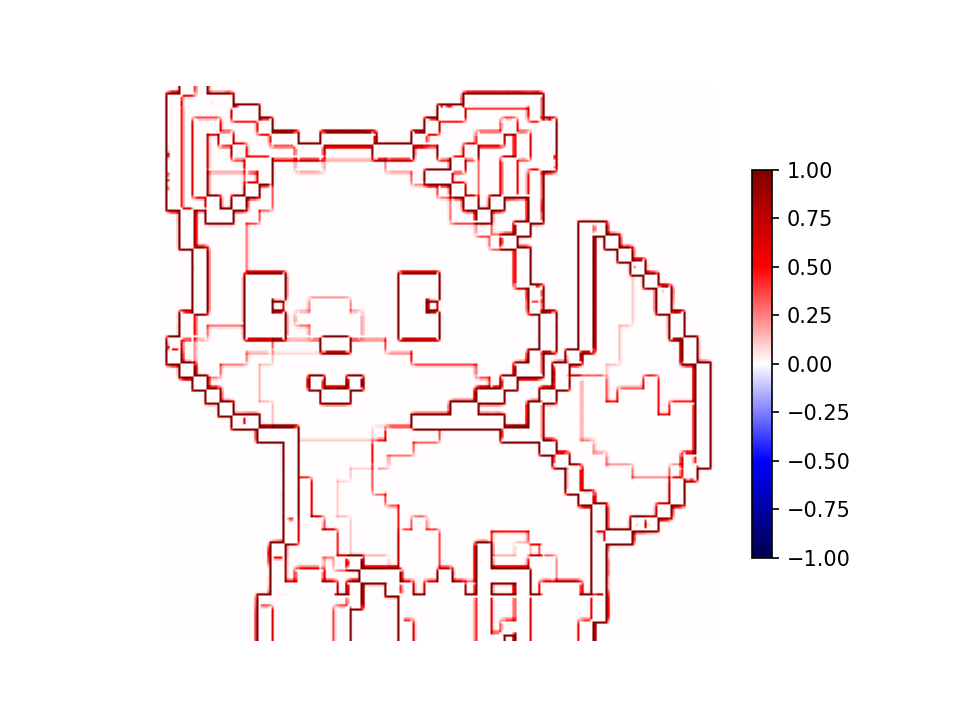
\includegraphics[width=0.6\textwidth]{src/edge.png}
  \caption{Выделение краёв с \texttt{filter2D()}.}
  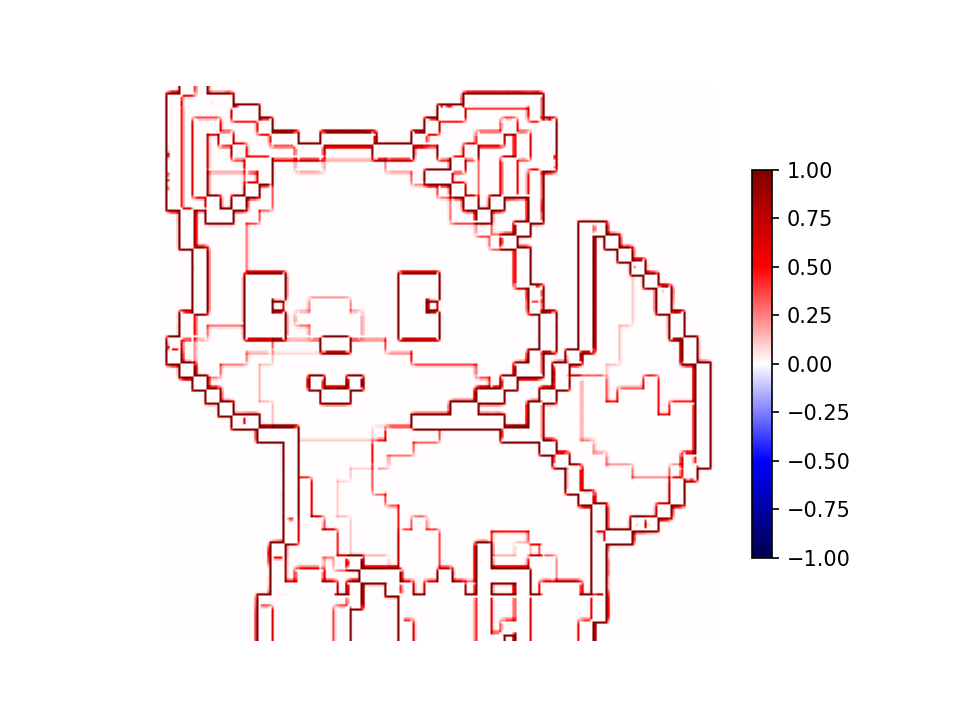
\includegraphics[width=0.6\textwidth]{src/ifft_edge.png}
  \caption{Выделение краёв через Фурье-образ.}
\end{figure}
\noindent Результат аналогичен. Посмотрим на образ отфильтрованного изображения:
\begin{figure}[H]
  \centering
  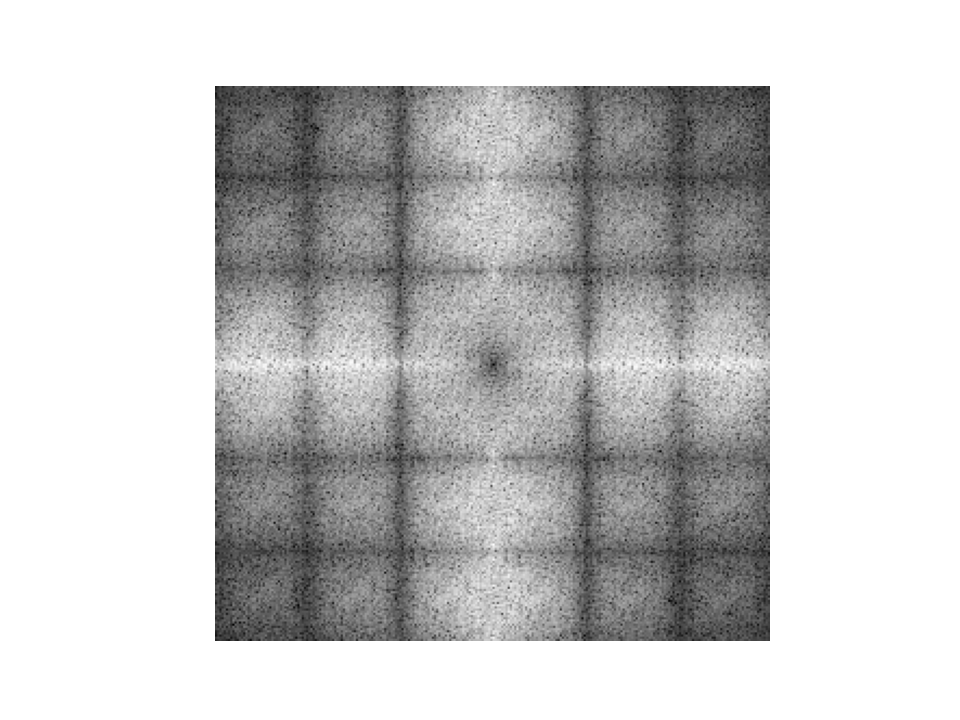
\includegraphics[width=0.6\textwidth]{src/ifft_spec_edge.png}
  \caption{Образ отфильтрованного изображения.}
\end{figure}
\noindent Мы видим, что прямые в вертикали и горизонтали становятся ярче, высокочастотные компоненты также светлеют, однако центральный пик обнуляется и становится черным. Это происходит потому что фильтр выделения краёв усиливает высокочастотные компоненты, которые отвечают за резкость изображения.

Теперь попробуем последний — кастомный фильтр Собеля. Применим его и посмотрим на результат:
\begin{figure}[H]
  \centering
  
\includegraphics[width=0.4\textwidth]{src/grayscale.png}
  \caption{Исходное изображение.}  
  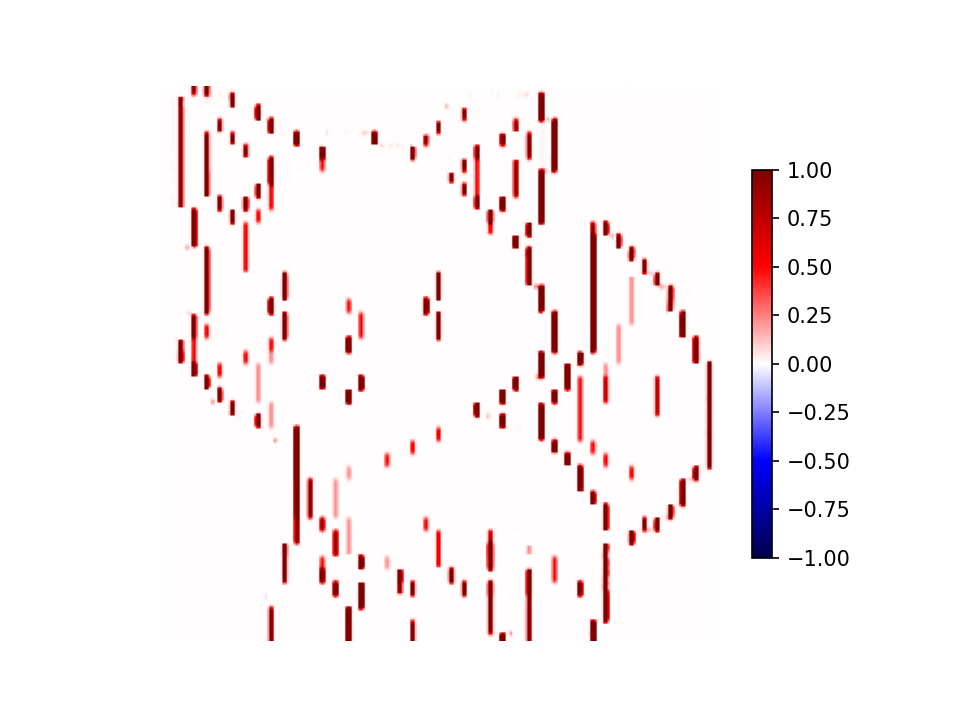
\includegraphics[width=0.7\textwidth]{src/custom.png}
  \caption{Фильтр Собеля с \texttt{filter2D()}.}
\end{figure}
\noindent Мы видим, что границы изображения по вертикали стали четкими. Посмотрим на образ ядра фильтра:
\begin{figure}[H]
  \centering
  \includesvg[width=0.4\textwidth]{src/spec_custom.svg}
  \caption{Образ ядра фильтра Собеля.}
\end{figure}  
\noindent Мы видим, что ядро фильтра имеет темный пик в центре в виде вертикальной прямой и мягкие переходы между участками. Теперь попробуем применить тот же фильтр, но вторым способом. 
\begin{figure}[H]
  \centering
  \includegraphics[width=0.6\textwidth]{src/custom.png}
  \caption{Фильтр Собеля с \texttt{filter2D()}.}
  \includegraphics[width=0.6\textwidth]{src/ifft_custom.png}
  \caption{Кастомный фильтр Собеля через Фурье-образ.}
\end{figure}
\noindent Результат аналогичен. Посмотрим на образ отфильтрованного изображения:
\begin{figure}[H]
  \centering
  \includegraphics[width=0.6\textwidth]{src/ifft_spec_custom.png}
  \caption{Образ отфильтрованного изображения.}
\end{figure}
\noindent Мы видим, что в этом случае становится ярче только горизонтальная прямая, а вертикальная прямая полностью пропадает. Это позволяет чётко выявлять вертикальную структуру без излишнего усиления шума. 

\paragraph{Выводы}
\begin{itemize}
  \item Для всех использованных ядер (гауссовых, блочных, повышения резкости, выделения краёв и кастомных) результаты пространственной свёртки и метода умножения спектров совпадают.
  \item Гауссово размытие демонстрирует плавные радиально-симметричные переходы без артефактов геометрии окна; с ростом размера ядра $N$ область низких частот сужается, а высокие частоты подавляются всё сильнее.
  \item Блочное размытие создаёт «мозаичный» эффект: внутри каждого окна яркость усредняется одинаково, при больших $N$ образуются ступенчатые плато и резкие границы между ними.
  \item Ядро повышения резкости подчёркивает высокочастотные компоненты, делая контуры ощутимо более чёткими, при этом сохраняется средняя яркость.
  \item Ядро выделения краёв усиливает перепады яркости, обнуляя «низкие» частоты и показывая тонкие границы.
  \item Кастомное ядро — оператор Собеля по $x$ — позволяет выделять границы в заданном направлении, что полезно для анализа текстур и ориентации структур на изображении.
  \item Путём выбора формы ядра и его параметров можно получать широкий спектр фильтров: от низкочастотного сглаживания до направленного детектирования контуров и сложных текстурных эффектов.
\end{itemize}

\addsection{Выводы}
\begin{itemize}
  \item FFT-фильтрация позволила наглядно обнаружить и «заглушить» периодические артефакты в спектре изображения, сохранив при этом фазу и среднюю яркость, что дало чистый результат без контрастных искажений.
  \item Пространственная и частотная свёртки дали совпадающие результаты при корректном центрировании ядра и обрезке, подтвердив теорему о свёртке.
  \item Гауссово размытие обеспечивает плавное подавление высоких частот, а блочное - ступенчатое усреднение.
  \item Фильтры резкости, выделения краёв дают широкий спектр эффектов: от подчёркивания границ до выделения текстур.
  \item Подбор ядра позволяет гибко управлять результатом фильтрации.
\end{itemize}

\pagebreak
\addsection{Приложение}
\begin{lstlisting}[caption={Исходный код}]
import numpy as np
from PIL import Image
import matplotlib.pyplot as plt
import cv2 as cv

def visualize(image, path=None, cmap=None, dpi=150, m=None):
    plt.figure(frameon=False, dpi=dpi)    
    plt.axis('off')
    if m is not None:
        im = plt.imshow(image, cmap=cmap, vmin=-m, vmax=+m)
        plt.colorbar(im, shrink=0.7)
    elif image.ndim == 2:
        plt.imshow(image, cmap=cmap, vmin=0, vmax=1)
    else:
        plt.imshow(image)
    if path is not None:
        plt.savefig(path)
    plt.show()

def compute_spec(img):
    F = np.fft.fftshift(np.fft.fft2(img, axes=(0,1)), axes=(0,1))
    phase = np.angle(F)
    F_abs = np.abs(F)
    log_mag = np.log(F_abs + 1)
    log_max = log_mag.max()
    log_norm = log_mag / log_max
    return log_norm, phase, log_max

def reconstruct_image(log_norm, phase, log_max):
    F_complex = np.exp(1j * phase) * (np.exp(log_norm * log_max) - 1)
    rec = np.fft.ifft2(np.fft.ifftshift(F_complex, axes=(0,1)), axes=(0,1))
    rec = rec.real
    rec = np.clip(rec, 0, 1)
    return rec

    def gaussian_kernel(n):
    sigma = (n - 1) / 6.0
    A = np.array([[np.exp(-((i - (n + 1) / 2) ** 2 + (j - (n + 1) / 2) ** 2) /  (2 * sigma ** 2)) for i in range(1, n + 1)] for j in range(1, n + 1)])
    return A / A.sum()

def box_kernel(n):
    A = np.ones((n, n), dtype=float)
    return A / A.sum()

def sharpen_kernel():
    return np.array([[0, -1, 0],
                      [-1, 5, -1],
                      [0, -1, 0]], dtype=float)

def edge_kernel():
    return np.array([[-1, -1, -1],
                      [-1, 8, -1],
                      [-1, -1, -1]], dtype=float)

def custom_kernel():
    return np.array([[-1, 0, 1],
                      [-2, 0, 2],
                      [-1, 0, 1]], dtype=float)

def make_kernels():
    kernels = []
    for N in (9, 15, 49):
        kernels.append((gaussian_kernel(N), f'gauss_{N}'))
    for N in (9, 15, 49):
        kernels.append((box_kernel(N), f'box_{N}'))
    kernels.append((sharpen_kernel(), 'sharpen'))
    kernels.append((edge_kernel(), 'edge'))
    kernels.append((custom_kernel(), 'custom'))
    return kernels

    def apply_spatial_kernels(image, kernels, out_dir=None):
    for kernel, name in kernels:
        filtered = cv.filter2D(image, ddepth=-1, kernel=kernel)
        log_norm = kernel_spectrum(kernel, image.shape)
        if name not in ['sharpen', 'edge', 'custom']:
            visualize(filtered, path=f"{out_dir}/{name}.png" if out_dir else None, cmap='gray')
        else:
            filtered = filtered.clip(0, 1)
            if name in ['edge', 'custom']:
                m = np.max(np.abs(filtered))
                visualize(filtered, path=f"{out_dir}/{name}.png" if out_dir else None, cmap='seismic', m=m)
            else:
                visualize(filtered, path=f"{out_dir}/{name}.png" if out_dir else None, cmap='gray')
        visualize(log_norm, path=f"{out_dir}/spec_{name}.svg" if out_dir else None, cmap='gray')


def apply_frequency_kernels(image, kernels, out_dir=None):
    h, w = image.shape
    for K, name in kernels:
        kh, kw = K.shape
        ph, pw = kh//2, kw//2
        I_pad = np.pad(image, ((ph,ph),(pw,pw)), mode='reflect')

        H, W = I_pad.shape
        K = np.flipud(np.fliplr(K))

        F_i = np.fft.fft2(I_pad)
        F_k = np.fft.fft2(K, s=(H,W))

        conv_full = np.fft.ifft2(F_i * F_k).real

        conv = conv_full[kh - 1:kh+h, kw - 1:kw+w]        
        
        log_norm, _, _ = compute_spec(conv)
        if name not in ['sharpen', 'edge', 'custom']:
            visualize(conv, path=f"{out_dir}/ifft_{name}.png" if out_dir else None, cmap='gray')
        else:
            conv = conv.clip(0, 1)
            if name in ['edge', 'custom']:
                m = np.max(np.abs(conv))
                visualize(conv, path=f"{out_dir}/ifft_{name}.png" if out_dir else None, cmap='seismic', m=m)
            else:
                visualize(conv, path=f"{out_dir}/{name}.png" if out_dir else None, cmap='gray')
        visualize(log_norm, path=f"{out_dir}/ifft_spec_{name}.png" if out_dir else None, cmap='gray')


def task1(image_path):
    img = Image.open(image_path).convert('RGB')
    img_arr = np.asarray(img, dtype=np.float64) / 255.0

    log_norm, phase, log_max = compute_spec(img_arr)
    visualize(log_norm, path='src/spec_orig.png', cmap='gray')

    edited = Image.open('src/spec_filtered.png').convert('RGB')
    edited_arr = np.asarray(edited, dtype=np.float64) / 255.0

    rec = reconstruct_image(edited_arr, phase, log_max)
    visualize(img_arr)
    visualize(rec, path='src/filtered.png')

def task2(path):
    img = Image.open(path).convert('L')
    img_arr = np.asarray(img, dtype=np.float64) / 255.0
    visualize(img_arr, cmap='gray', path='src/grayscale.png')

    log_norm, phase, log_max = compute_spec(img_arr)
    visualize(log_norm, path='src/spec_pixel.png', cmap='gray')

    kernels = make_kernels()
    apply_spatial_kernels(img_arr, kernels, out_dir='src')
    apply_frequency_kernels(img_arr, kernels, out_dir='src')

task1('src/13.png')
task2('src/pixel.png')
\end{lstlisting}
\end{document}